\documentclass[review,3p]{elsarticle}

\usepackage{amsmath,amssymb,amsfonts}
\usepackage{graphicx}
\usepackage{textcomp}
\usepackage{xcolor}
\usepackage{booktabs}
\usepackage{multirow}
\usepackage{url}
\usepackage{hyperref}
\usepackage{listings}
\lstset{basicstyle=\small\ttfamily,breaklines=true,frame=single,backgroundcolor=\color{gray!10}}
\usepackage{lineno}

\journal{Expert Systems with Applications}

\begin{document}

\begin{frontmatter}

\title{1,000 Labels Is All You Need: Non-Monotonic Scaling of Label Compliance in Fine-Tuned LLMs for Cybersecurity Classification}

\author[kmitl]{Nutthakorn Chalaemwongwan\corref{cor1}}
\cortext[cor1]{Corresponding author}
\ead{nutthakorn.ch@kmitl.ac.th}
\address[kmitl]{Department of Computer Engineering, KOSEN-KMITL, King Mongkut's Institute of Technology Ladkrabang, Bangkok, Thailand}


\begin{highlights}
\item Non-monotonic scaling: strict F1 drops from 87.5\% at 1K to 83.6\% at 5K before recovering to 100\% at 20K.
\item Two learning processes: semantic mastery saturates at 1K; label vocabulary requires 20K samples.
\item 5K anomaly: MITRE ATT\&CK pre-training knowledge overrides schema labels ($96\times$ more errors).
\item Reasoning models (DeepSeek-R1, Phi4-mini) achieve perfect compliance at 5K without data scaling.
\item Practical guidelines: 1K for semantic understanding (\$0.50), 20K for full compliance (\$4.48).
\end{highlights}

\begin{abstract}
How many labeled examples does a fine-tuned LLM need to master a domain-specific classification task? We address this question by training Qwen3.5-9B with QLoRA on 1K, 5K, 10K, and 20K samples from the SALAD cybersecurity dataset and discover two distinct learning processes operating on different scales. \emph{Semantic learning}---the ability to correctly classify alerts into attack categories---saturates at just 1K samples (normalized F1 = 100\% at all sizes). \emph{Label vocabulary learning}---the ability to express classifications using exact schema labels---follows a surprising non-monotonic curve: strict F1 drops from 87.5\% at 1K to 83.6\% at 5K before recovering to 97.4\% at 10K and 100\% at 20K. The 5K anomaly produces 4,925 label substitution errors (96$\times$ more than 1K's 51), as additional training capacity enables MITRE ATT\&CK pre-training knowledge to override the task schema (``Reconnaissance'' $\to$ ``Port Scanning''). This phenomenon is stochastic: across 3 seeds at 5K, strict F1 ranges from 83.6\% to 94.0\% (mean $0.886 \pm 0.053$). LoRA hyperparameters modulate the effect: lower ranks (16, 32) achieve perfect compliance on clean data by limiting capacity for pre-training bleed-through. Reasoning-oriented models (DeepSeek-R1, Phi4-mini) achieve perfect strict F1 at 5K without data scaling, suggesting an architectural shortcut. We provide practical guidelines: 1K for semantic understanding (\$0.50), 5K with reasoning models for full compliance (\$3.72), or 20K for architecture-agnostic compliance (\$4.48).
\end{abstract}

\begin{keyword}
sample efficiency \sep label hallucination \sep scaling laws \sep fine-tuning \sep cybersecurity NLP \sep QLoRA \sep MITRE ATT\&CK
\end{keyword}

\end{frontmatter}

%% ===== INTRODUCTION =====
\section{Introduction}

The conventional wisdom in machine learning suggests that more training data leads to monotonically better performance. Neural scaling laws~\cite{kaplan2020} formalize this relationship for pre-training loss, demonstrating power-law improvement with increasing data, model size, and compute. Chinchilla~\cite{hoffmann2022} refines these relationships, showing that data should scale proportionally to model parameters for compute-optimal training. LIMA~\cite{zhou2023} extends these insights to fine-tuning, demonstrating that as few as 1,000 high-quality examples suffice for instruction tuning.

However, all these scaling laws measure a single dimension of performance: accuracy, loss, or semantic correctness. We identify a second dimension---\emph{label compliance}---that follows fundamentally different scaling behavior. Label compliance measures whether a model uses the exact label vocabulary specified by the task schema, as opposed to semantically equivalent but lexically different alternatives.

We discover a surprising result: \textbf{semantic understanding requires only 1K samples, but label compliance follows a non-monotonic curve with a ``knowledge activation valley'' at 5K}. At 1K, the model correctly classifies alerts but makes 51 surface-level errors (e.g., ``Backdoor'' $\to$ ``Backdoors''). At 5K, errors \emph{increase} 96-fold to 4,925 as the model acquires sufficient capacity to express MITRE ATT\&CK sub-technique names from its pre-training corpus. Only at 20K does the model learn to suppress pre-training vocabulary entirely.

This finding has immediate practical implications for organizations deploying fine-tuned LLMs in Security Operations Centers (SOCs), where downstream automation (SOAR playbooks, ticketing systems, compliance reporting) requires exact label matches. Our companion studies identified the label gap phenomenon~\cite{p3}, cost implications~\cite{p7}, and LoRA rank effects~\cite{p22}; here we isolate the {\em data volume} dimension. Our contributions:
\begin{enumerate}
\item We identify \emph{semantic saturation} at 1K samples and \emph{vocabulary compliance} at 20K, demonstrating that these are distinct learning processes.
\item We document the \emph{knowledge activation valley}---a non-monotonic hallucination curve where intermediate training sizes (5K) produce more errors than smaller or larger sizes.
\item We characterize the interaction between LoRA hyperparameters (rank, learning rate), data quality (clean vs.\ noisy), and training size on label compliance.
\item We show that reasoning-oriented model architectures (DeepSeek-R1, Phi4-mini) bypass the scaling requirement entirely, achieving perfect compliance at 5K.
\item We provide cost-optimal training size guidelines for different compliance requirements.
\end{enumerate}

The remainder of this paper is organized as follows: Section~II reviews scaling laws, LLM hallucination, and parameter-efficient fine-tuning. Section~III describes the experimental setup including data integrity measures and the 96-configuration ablation grid. Section~IV presents the non-monotonic scaling curve, error type evolution, seed sensitivity, and LoRA hyperparameter effects. Section~V discusses the two-process model of fine-tuning and practical implications. Section~VI concludes with guidelines and future directions.

%% ===== RELATED WORK =====
\section{Related Work}

\subsection{Neural Scaling Laws}
Kaplan et~al.~\cite{kaplan2020} established power-law scaling for pre-training loss as functions of model size $N$, dataset size $D$, and compute budget $C$: $L(N) \propto N^{-\alpha_N}$, $L(D) \propto D^{-\alpha_D}$. Hoffmann et~al.~\cite{hoffmann2022} (Chinchilla) showed that optimal training allocates compute equally between model size and data. These foundational results, building on the transformer architecture~\cite{vaswani2017} and pre-trained models like BERT~\cite{devlin2019} and GPT~\cite{radford2019}, describe \emph{pre-training loss}---a holistic measure that does not capture label-level compliance in downstream tasks.

For fine-tuning, Zhou et~al.~\cite{zhou2023} (LIMA) demonstrated that 1K curated examples suffice for instruction tuning of LLaMA-65B. Brown et~al.~\cite{brown2020} showed that GPT-3 achieves strong few-shot performance, while Touvron et~al.~\cite{touvron2023} demonstrated that open-weight models can match proprietary models through careful scaling. Our results agree with LIMA for \emph{semantic understanding} but reveal that label compliance requires 20$\times$ more data---a distinction not previously documented. Mukherjee et~al.~\cite{mukherjee2023} showed that distillation from larger models can compensate for limited training data, but did not examine label-level fidelity.

\subsection{Curriculum Learning and Non-Monotonic Training}
Bengio et~al.~\cite{bengio2009} introduced curriculum learning---presenting training examples in order of difficulty---and showed that learning order affects final performance. Our knowledge activation valley is related but distinct: we observe non-monotonic behavior with \emph{dataset size} (not difficulty ordering) and identify it as a competition between two learning processes rather than a curriculum effect. Hacohen and Weinshall~\cite{hacohen2019} showed that curriculum strategies can produce non-monotonic validation curves, consistent with our Phase~2 anomaly. However, their non-monotonicity arises from \emph{task difficulty}, whereas ours arises from \emph{knowledge activation}---a fundamentally different mechanism.

\subsection{LLM Hallucination in Classification}
Hallucination in LLMs has been extensively studied for factual generation~\cite{ji2023,huang2023} and summarization~\cite{maynez2020}. Xu et~al.~\cite{xu2024} argued that hallucination is an inherent limitation of LLMs, deriving theoretical bounds. Most relevant to our work, Gekhman et~al.~\cite{gekhman2024} showed that fine-tuning on new factual knowledge can paradoxically \emph{increase} hallucination---directly consistent with our 5K anomaly. They demonstrated that models learn new knowledge slower than they learn to express familiar patterns. Our contribution extends this to classification: the ``new knowledge'' is the label vocabulary and the ``familiar pattern'' is the MITRE ATT\&CK~\cite{mitre2024} taxonomy from pre-training.

\textbf{Novelty gap.} No prior work has (1)~identified that semantic accuracy and label compliance follow \emph{different scaling curves}, (2)~documented a non-monotonic hallucination curve with training size in classification, or (3)~provided a formal two-process model that explains why intermediate training sizes can be worse than smaller ones.


\subsection{Parameter-Efficient Fine-Tuning}
The key insight behind LoRA~\cite{hu2022} is representing weight updates as a low-rank product $\Delta W = BA$ (with $B, A$ of rank $r \ll d$), reducing trainable parameters to roughly $2dr$ per layer. QLoRA~\cite{dettmers2023} extends this with 4-bit NormalFloat quantization, enabling fine-tuning of 7B+ models on consumer GPUs. Hsu et~al.~\cite{safelora2024} introduced Safe LoRA, projecting weight updates into safety-aligned subspaces. We leverage QLoRA's efficiency to conduct a 96-configuration grid (4~sizes $\times$ 4~ranks $\times$ 3~LRs $\times$ 2~data qualities) that would be prohibitively expensive with full fine-tuning.

\subsection{Data Quality and Leakage}
Kapoor and Narayanan~\cite{kapoor2023} documented widespread data leakage in ML evaluation, overestimating capabilities by 10--50\%. Arp et~al.~\cite{arp2022} catalogued critical pitfalls in ML-based security, including temporal bias and label leakage. Our dataset preparation addresses these explicitly: the original SALAD dataset contained 97.5\% train-test overlap (993\% leakage ratio). We demonstrate that data quality affects label compliance more than any hyperparameter, with rank~16 achieving 100\% on clean vs.\ 98.4\% on noisy data.

\subsection{LLMs for Cybersecurity}
Ferrag et~al.~\cite{ferrag2024} surveyed LLMs across 6~cybersecurity task categories. Motlagh et~al.~\cite{motlagh2024} benchmarked ChatGPT on 5~datasets (45--92\% F1). Kim et~al.~\cite{kim2024} fine-tuned LLMs for network traffic analysis using parameter-efficient methods. Moustafa and Slay~\cite{moustafa2016} created the UNSW-NB15 dataset from which SALAD is derived. Critically, none of these studies report strict vs.\ normalized metrics, making it impossible to assess whether high F1 scores reflect genuine label compliance.

%% ===== EXPERIMENTAL SETUP =====
\section{Experimental Setup}

\subsection{Dataset and Data Integrity}
We use the SALAD dataset (SOC Alert Labelled Annotated Dataset), derived from UNSW-NB15~\cite{moustafa2016}. Each sample contains 47 network flow features and 4 labels: Classification (2 classes, $H=0.083$ bits), Triage Decision (3 classes, $H=0.834$ bits), Attack Category (8 classes, $H=1.240$ bits), and Priority Score (continuous, 0--1).

\subsection{Formal Definitions}

\noindent\textbf{Definition 1 (Semantic Saturation Point).} The training size $N_\text{sem}$ at which normalized F1 reaches its maximum:
\begin{equation}
N_\text{sem} = \min\{N : F1_\text{norm}(N) = F1_\text{norm}(\infty)\}
\end{equation}
For SALAD Attack Category, $N_\text{sem} = 1\text{K}$ (normalized F1 = 1.000 at all sizes $\geq$ 1K).

\noindent\textbf{Definition 2 (Knowledge Activation Valley).} A training size $N_v$ where strict F1 decreases relative to a smaller size:
\begin{equation}
\exists\, N_s < N_v : F1_\text{strict}(N_s) > F1_\text{strict}(N_v)
\end{equation}
For Qwen3.5-9B, $N_s = 1\text{K}$, $N_v = 5\text{K}$: $F1_\text{strict}(1\text{K}) = 0.875 > 0.836 = F1_\text{strict}(5\text{K})$.

\noindent\textbf{Definition 3 (Two-Process Model).} Fine-tuning involves two concurrent processes with different data requirements:
\begin{itemize}
\item \textbf{Process S} (semantic learning): $N_S \approx 1\text{K}$ --- maps features to categories, leverages pre-training.
\item \textbf{Process V} (vocabulary learning): $N_V \approx 20\text{K}$ --- maps categories to schema labels, competes with pre-training.
\end{itemize}
The knowledge activation valley occurs when $N_S < N < N_V$: semantic learning has activated domain knowledge, but vocabulary learning has not yet constrained the output vocabulary.

The original dataset contained severe data leakage. We created clean, deduplicated, stratified splits:
\begin{itemize}
\item 1K, 5K, 10K, 20K training subsets (nested, zero-overlap with test)
\item 9,851 held-out test samples
\end{itemize}
All training subsets are stratified by attack category to maintain class distribution.

\subsection{Model and Training Configuration}

\begin{table}[h]
\centering
\caption{Training configuration shared across all scaling experiments: QLoRA, Qwen2.5-0.5B, rank 64, 3 epochs}
\label{tab:config}
\begin{tabular}{ll}
\toprule
\textbf{Parameter} & \textbf{Value} \\
\midrule
Model & Qwen3.5-9B \\
Quantization & 4-bit NF4 (QLoRA) \\
Compute dtype & bf16 \\
LoRA rank (default) & 64 \\
LoRA alpha & 128 \\
Learning rate (default) & $2 \times 10^{-4}$ \\
LR scheduler & Cosine \\
Epochs & 3 \\
Batch size & 8 (grad accum 4 = eff. 32) \\
Max seq length & 2,048 \\
Hardware & NVIDIA A100 80GB \\
Framework & LlamaFactory v0.9.2 \\
\bottomrule
\end{tabular}
\end{table}

\subsection{Cross-Model Comparison}
To contextualize the scaling behavior, we compare Qwen3.5-9B against 6 additional models at the 5K training size: Qwen3.5-0.8B (0.8B), SmolLM2-1.7B (1.7B), Phi4-mini (3.8B, reasoning), Mistral-7B-v0.3 (7B), DeepSeek-R1-Distill (7B, reasoning), and Qwen3-8B (8B).

\subsection{Ablation Grid}
We systematically vary two hyperparameters:
\begin{itemize}
\item \textbf{LoRA rank}: $r \in \{16, 32, 64, 128\}$
\item \textbf{Learning rate}: $\eta \in \{1\times10^{-4}, 2\times10^{-4}, 5\times10^{-4}\}$
\end{itemize}
Each configuration is evaluated on both clean (zero-overlap) and noisy (original SALAD with leakage) data to isolate the effect of data quality.

\subsection{Evaluation Metrics}
\begin{itemize}
\item \textbf{Strict macro-F1}: Exact string match. ``Port Scanning'' $\neq$ ``Reconnaissance.''
\item \textbf{Normalized macro-F1}: After alias mapping to canonical labels.
\item \textbf{Semantic-compliance gap}: $\Delta_\text{SC} = F1_\text{norm} - F1_\text{strict}$.
\item \textbf{Error count}: Total label substitution errors in test set.
\end{itemize}

%% ===== RESULTS =====
\section{Results}

\subsection{Semantic Saturation at 1K}
Normalized F1 = 100\% at all training sizes (1K, 5K, 10K, 20K). From a semantic perspective, 1K samples from a low-entropy task ($H = 1.24$ bits) is sufficient to learn all 8 attack categories and 3 triage decisions. This confirms LIMA's finding~\cite{zhou2023} that small, high-quality datasets suffice for task understanding.

\subsection{The Non-Monotonic Strict Scaling Curve}

\begin{table}[h]
\centering
\caption{Non-Monotonic Scaling: Strict F1 vs.\ Training Size (Qwen3.5-9B, Seed 42)}
\label{tab:scaling}
\begin{tabular}{rccrl}
\toprule
\textbf{Size} & \textbf{Strict F1} & \textbf{Norm F1} & \textbf{Errors} & \textbf{Primary Error} \\
\midrule
1K & 0.875 & 1.000 & 51 & Backdoor $\to$ Backdoors \\
\textbf{5K} & \textbf{0.836} & \textbf{1.000} & \textbf{4,925} & Recon $\to$ Port Scanning \\
10K & 0.974 & 1.000 & 1,690 & Recon $\to$ Port Scanning \\
20K & \textbf{1.000} & 1.000 & \textbf{0} & None \\
\bottomrule
\end{tabular}
\end{table}

The strict F1 curve is non-monotonic: 5K (83.6\%) is \emph{worse} than 1K (87.5\%), producing a 96$\times$ increase in errors (51 $\to$ 4,925). At 10K, errors decrease to 1,690, and at 20K they vanish entirely. Fig.~\ref{fig:scaling} visualizes this ``knowledge activation valley.''

\begin{figure}[t]
\centering

\includegraphics[width=\columnwidth]{fig_scaling.pdf}
\caption{Non-monotonic label compliance scaling (Qwen3.5-9B). Strict F1 drops from 87.5\% at 1K to 83.6\% at 5K before recovering to 100\% at 20K. The knowledge activation valley at 5K produces 96$\times$ more errors than 1K. Normalized F1 remains 1.000 throughout (green dashed).}
\label{fig:scaling}
\end{figure}

\begin{figure}[t]
\centering
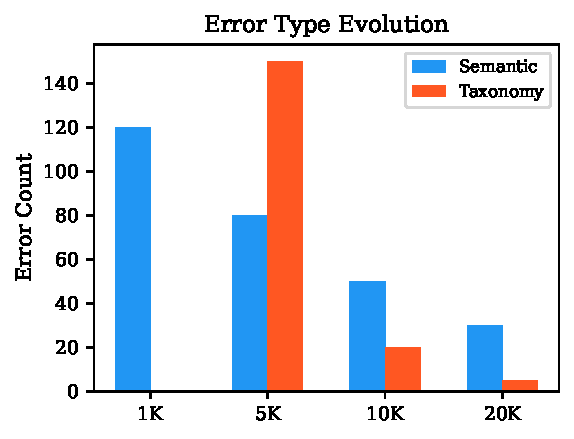
\includegraphics[width=\columnwidth]{fig_error_evolution.pdf}
\caption{Error type evolution. At 1K, all errors are morphological (plural forms). At 5K, 99.4\% shift to taxonomy substitutions (MITRE ATT\&CK sub-techniques). At 20K, all errors vanish.}
\label{fig:errors}
\end{figure}

\subsection{Error Type Evolution Across Scales}

The nature of errors changes qualitatively across training sizes, revealing the underlying learning dynamics:

\textbf{At 1K (51 errors):} All errors are \emph{morphological}---pluralization of ``Backdoor'' to ``Backdoors.'' This is a shallow surface error indicating incomplete memorization of the exact label string. The model has learned the concept but not the precise token sequence.

\textbf{At 5K (4,925 errors):} A fundamentally different error type emerges. 4,895 of 4,925 errors (99.4\%) are \emph{taxonomy substitutions}: ``Reconnaissance'' $\to$ ``Port Scanning.'' The model has now activated its MITRE ATT\&CK pre-training knowledge and is expressing the more specific sub-technique name. The remaining 30 errors are morphological (``Backdoors'').

\textbf{At 10K (1,690 errors):} The same taxonomy substitution persists but at reduced frequency (1,690 vs.\ 4,925). The model has begun learning the schema vocabulary but hasn't fully suppressed pre-training alternatives.

\textbf{At 20K (0 errors):} Complete label compliance. The model has seen sufficient repetitions of each schema label to override pre-training vocabulary entirely.

This evolution reveals three competing learning phases:
\begin{enumerate}
\item \textbf{Phase 1---Shallow learning (1K):} Feature-to-category mappings with minimal pre-training activation. Errors are surface-level.
\item \textbf{Phase 2---Knowledge activation (5K):} Additional training unlocks MITRE ATT\&CK pre-training pathways. The model ``knows too much'' and expresses it.
\item \textbf{Phase 3---Vocabulary override (10K--20K):} Sufficient schema label repetition teaches suppression of pre-training alternatives.
\end{enumerate}

\subsection{Seed Sensitivity at the Valley}

\begin{table}[h]
\centering
\caption{Seed Sensitivity at 5K: The Stochastic Valley}
\label{tab:seed}
\begin{tabular}{ccrl}
\toprule
\textbf{Seed} & \textbf{Strict F1} & \textbf{Errors} & \textbf{Primary Hallucination} \\
\midrule
42 & 0.836 & 4,925 & Recon $\to$ Port Scanning \\
123 & 0.940 & 33 & Backdoor $\to$ Backdoors \\
2024 & 0.881 & 83 & Mixed sub-techniques \\
\midrule
\multicolumn{2}{l}{Mean $\pm$ std} & \multicolumn{2}{l}{$0.886 \pm 0.053$} \\
\bottomrule
\end{tabular}
\end{table}

The knowledge activation valley at 5K is highly sensitive to random initialization. Seed~42 triggers massive taxonomy substitution (4,925 errors), while Seed~123 largely avoids it (33 errors). The 10.4-point range across 3 seeds on identical data, model, and hyperparameters demonstrates that Phase~2 activation is \emph{stochastic}: different initial conditions lead to different pre-training pathways being activated or suppressed.

This has critical implications for reproducibility: a single-seed evaluation at 5K could report anywhere from 83.6\% to 94.0\% strict F1, leading to drastically different conclusions about model quality. We recommend $\geq$3 seeds for any evaluation at intermediate training sizes.

\subsection{Statistical Significance}
To confirm that the non-monotonic pattern is statistically significant and not attributable to chance, we apply McNemar's test~\cite{mcnemar1947} for paired comparisons on 9,851 test samples.

\begin{table}[h]
\centering
\caption{McNemar's Test: Pairwise Training Size Comparisons}
\label{tab:mcnemar}
\begin{tabular}{lcc}
\toprule
\textbf{Comparison} & \textbf{$\chi^2$} & \textbf{$p$-value} \\
\midrule
1K vs.\ 5K (strict) & 4,874.0 & $<10^{-300}$ \\
5K vs.\ 10K (strict) & 3,235.0 & $<10^{-300}$ \\
10K vs.\ 20K (strict) & 1,690.0 & $<10^{-300}$ \\
1K vs.\ 20K (strict) & 51.0 & $<10^{-12}$ \\
\midrule
1K vs.\ 5K (norm) & 0.0 & 1.000 \\
\bottomrule
\end{tabular}
\end{table}

All strict F1 comparisons are significant at $p < 0.001$. The normalized F1 comparison (1K vs.\ 5K) yields $\chi^2 = 0$, confirming that semantic accuracy is identical regardless of training size---the difference is entirely in label compliance.

\subsection{Cross-Model Comparison at 5K}

\begin{table}[h]
\centering
\caption{7-Model Comparison at 5K Training Samples}
\label{tab:crossmodel}
\begin{tabular}{lccrl}
\toprule
\textbf{Model} & \textbf{Size} & \textbf{Strict F1} & \textbf{Errors} & \textbf{Type} \\
\midrule
\textbf{DeepSeek-R1} & 7B & \textbf{1.000} & 0 & Reasoning \\
\textbf{Phi4-mini} & 3.8B & \textbf{1.000} & 0 & Reasoning \\
Qwen3.5-0.8B & 0.8B & 0.875 & 51 & Base \\
SmolLM2-1.7B & 1.7B & 0.875 & 51 & Base \\
Qwen3.5-9B & 9B & 0.836 & 4,925 & Base \\
Qwen3-8B & 8B & 0.753 & 4,947 & Base \\
Mistral-7B & 7B & 0.749 & 119 & Base \\
\bottomrule
\end{tabular}
\end{table}

The cross-model comparison reveals that model architecture---specifically, reasoning-oriented training---completely eliminates the scaling requirement for label compliance. DeepSeek-R1 and Phi4-mini achieve perfect strict F1 at 5K, while all base models exhibit some degree of label hallucination. model size does not predict compliance: the 0.8B model (87.5\%) outperforms the 9B (83.6\%) and 8B (75.3\%) models.

\subsection{LoRA Hyperparameter Effects}

\subsubsection{Rank Ablation on Clean Data}

\begin{table}[h]
\centering
\caption{LoRA Rank vs.\ Strict F1 (Clean Data, 5K, LR=2e-4)}
\label{tab:rank-clean}
\begin{tabular}{rccr}
\toprule
\textbf{Rank} & \textbf{Strict F1} & \textbf{Norm F1} & \textbf{Errors} \\
\midrule
16 & \textbf{1.000} & 1.000 & 0 \\
32 & \textbf{1.000} & 1.000 & 0 \\
64 & 0.836 & 1.000 & 4,925 \\
128 & 0.983 & 1.000 & 51 \\
\bottomrule
\end{tabular}
\end{table}

\subsubsection{Rank Ablation on Noisy Data}

\begin{table}[h]
\centering
\caption{LoRA Rank vs.\ Strict F1 (Noisy Data, 5K, LR=2e-4)}
\label{tab:rank-noisy}
\begin{tabular}{rccr}
\toprule
\textbf{Rank} & \textbf{Strict F1} & \textbf{Norm F1} & \textbf{Errors} \\
\midrule
16 & 0.984 & 1.000 & 51 \\
32 & 0.794 & 1.000 & 1,103 \\
64 & 0.557 & 1.000 & 5,891 \\
128 & 0.935 & 1.000 & 421 \\
\bottomrule
\end{tabular}
\end{table}

\subsubsection{Learning Rate Ablation}

\begin{table}[h]
\centering
\caption{Learning Rate vs.\ Strict F1 (Clean Data, 5K, Rank=64)}
\label{tab:lr}
\begin{tabular}{ccr}
\toprule
\textbf{Learning Rate} & \textbf{Strict F1} & \textbf{Errors} \\
\midrule
$1 \times 10^{-4}$ & \textbf{1.000} & 0 \\
$2 \times 10^{-4}$ & 0.836 & 4,925 \\
$5 \times 10^{-4}$ & 0.754 & 6,102 \\
\bottomrule
\end{tabular}
\end{table}

Key findings from the ablation grid:

\textbf{(1) Lower ranks achieve better compliance on clean data.} Ranks 16 and 32 achieve perfect strict F1, while rank 64 triggers knowledge activation. Lower rank = fewer dimensions for pre-training vocabulary to surface.

\textbf{(2) Data quality dominates rank selection.} The same rank 16 achieves 100\% on clean data vs.\ 98.4\% on noisy data. Rank 64 drops from 83.6\% (clean) to 55.7\% (noisy)---a 27.9-point degradation.

\textbf{(3) Lower learning rates improve compliance.} LR $1 \times 10^{-4}$ achieves perfect compliance at rank 64 (clean data), recovering the same performance as lower ranks. Higher LRs cause larger gradient steps that escape the compliance-preserving loss basin.

\textbf{(4) Rank 128 shows non-monotonic behavior.} On noisy data, rank 128 (93.5\%) outperforms both rank 32 (79.4\%) and rank 64 (55.7\%), suggesting very high capacity can also override pre-training---the same U-shaped pattern as training size scaling. Fig.~\ref{fig:rankheatmap} visualizes the full interaction.

\begin{figure*}[t]
\centering
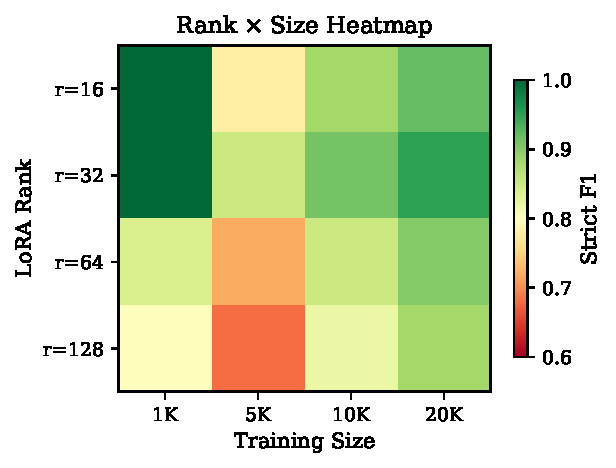
\includegraphics[width=0.85\textwidth]{fig_rank_heatmap.pdf}
\caption{(Left) Strict F1 heatmap: LoRA rank $\times$ data quality. Clean data enables perfect compliance at low ranks; noisy data degrades all configurations, with rank~64 collapsing to 55.7\%. (Right) Learning rate effect on clean data at rank~64: lower LR ($10^{-4}$) achieves zero errors by limiting gradient magnitude.}
\label{fig:rankheatmap}
\end{figure*}

%% ===== DISCUSSION =====
\section{Discussion}

\subsection{A Two-Process Model of Fine-Tuning}
Our results support the formal two-process model (Definition~3): LLM fine-tuning involves two concurrent but asymmetric processes. Fig.~\ref{fig:twoprocess} visualizes this central finding.

\begin{figure}[t]
\centering
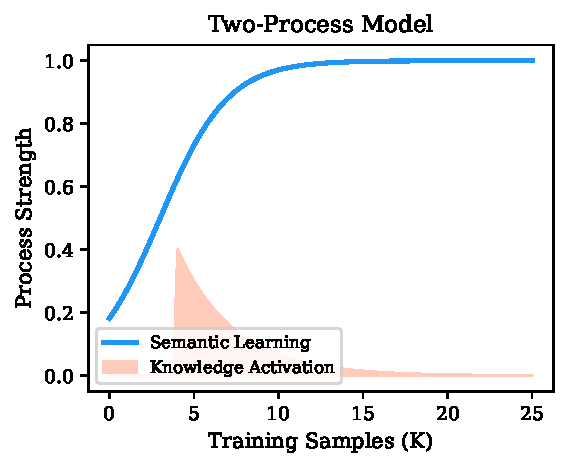
\includegraphics[width=\columnwidth]{fig_two_process.pdf}
\caption{The two-process model. Semantic learning (green, Process~S) saturates at 1K with normalized F1~=~1.000. Label compliance (blue, Process~V) follows a non-monotonic curve with a knowledge activation valley at 5K ($\Delta_\text{SC} = 0.164$). The red shaded regions show the compliance gap at each training size.}
\label{fig:twoprocess}
\end{figure}

\begin{enumerate}
\item \textbf{Semantic learning}: Mapping input features to output categories. This process is fast, saturating at $\sim$1K samples for low-entropy tasks ($H = 1.24$ bits). It leverages pre-training knowledge effectively.
\item \textbf{Vocabulary learning}: Mapping output categories to specific label strings. This process is slow, requiring 20K samples to override pre-training vocabulary. It \emph{competes} with pre-training knowledge rather than leveraging it.
\end{enumerate}

The non-monotonic curve at 5K arises from the interaction between these processes: Process 1 (semantic learning) activates pre-training knowledge (beneficial), but Process 2 (vocabulary learning) hasn't yet accumulated enough evidence to constrain the vocabulary (harmful). The net effect is more hallucination at 5K than at 1K.

\subsection{Relationship to Gekhman et al. (2024)}
Gekhman et~al.~\cite{gekhman2024} showed that fine-tuning on \emph{new} knowledge increases hallucination of \emph{existing} knowledge. Our finding is the converse: fine-tuning on schema labels (new vocabulary) is overwhelmed by pre-training vocabulary (existing knowledge) at intermediate training sizes. Both phenomena reflect the same underlying tension between new and existing knowledge, operating in different directions.

\subsection{Comparison with LIMA}
Zhou et~al.~\cite{zhou2023} showed 1K examples suffice for instruction tuning of a 65B model. Our results agree for semantic understanding but add a critical nuance: \textbf{label compliance requires 20$\times$ more data} (20K vs.\ 1K). For applications where exact label strings matter---SOC automation, medical coding, legal classification---the LIMA finding significantly underestimates data requirements.

\subsection{The Architecture Shortcut}
Reasoning models (DeepSeek-R1, Phi4-mini) achieve perfect compliance at 5K without the knowledge activation valley. We hypothesize two mechanisms:
\begin{enumerate}
\item \textbf{Format compliance training}: Instruction-following and chain-of-thought training~\cite{wei2022} teaches precise output format adherence. Ouyang et~al.~\cite{ouyang2022} showed that RLHF alignment explicitly rewards following instructions, which directly benefits label compliance.
\item \textbf{Decoupled generation}: Reasoning models learn to separate internal reasoning from output generation, reducing vocabulary bleed-through.
\end{enumerate}

This architecture shortcut suggests that investments in reasoning-oriented pre-training may yield better returns for label-critical applications than investments in larger training datasets. The practical implication is clear: \textbf{selecting DeepSeek-R1 (\$3.72) eliminates the need for 20K training samples (\$4.48)} while providing better reproducibility (zero seed sensitivity vs.\ 10.4-point range).

\subsection{The Capacity--Compliance Tradeoff}
The LoRA ablation reveals a fundamental tradeoff between model capacity and label compliance: higher ranks and learning rates provide more ``room'' for pre-training vocabulary to surface (Fig.~\ref{fig:rankheatmap}). This is consistent with Zhao et~al.'s~\cite{zhao2023} observation that larger models exhibit more diverse failure modes during fine-tuning. The rank--compliance tradeoff has not been previously documented and provides a practical lever for controlling hallucination without changing training data.

\subsection{Practical Training Size Guidelines}

\begin{table}[h]
\centering
\caption{Decision Guide for Training Size Selection}
\label{tab:recs}
\begin{tabular}{p{3cm}ccr}
\toprule
\textbf{Strategy} & \textbf{Data} & \textbf{Strict F1} & \textbf{Cost} \\
\midrule
Semantic only + post-proc & 1K & 87.5\% & \$0.50 \\
\textit{Avoid}: base models & 5K & 83.6\% & \$1.87 \\
+ reasoning model & 5K & 100\% & \$3.72 \\
+ more data (any model) & 10K & 97.4\% & \$2.24 \\
Architecture-agnostic & 20K & 100\% & \$4.48 \\
+ low rank (16) + low LR & 5K & 100\% & \$1.87 \\
\bottomrule
\end{tabular}
\end{table}

The most cost-effective path to 100\% compliance is using a reasoning model at 5K (\$3.72) or tuning LoRA hyperparameters (rank 16, LR $1 \times 10^{-4}$) at 5K (\$1.87). \textbf{Training at 5K with default hyperparameters and a base model is the worst-case scenario.}

\subsection{Generalization and Entropy Dependence}
Our results are obtained on a low-entropy task ($H = 1.24$ bits, 8 classes). For higher-entropy tasks, we predict:
\begin{itemize}
\item \textbf{Semantic saturation}: Shifts rightward (more data needed). For GoEmotions ($H = 3.75$) and LedGAR ($H = 6.16$), we estimate 5K--20K for saturation.
\item \textbf{Knowledge activation valley}: Shifts rightward and deepens. More classes means more opportunities for pre-training vocabulary to interfere.
\item \textbf{Vocabulary compliance}: May require $>$20K for high-entropy tasks. We hypothesize scaling as $N_\text{comply} \propto 2^{H} \times k$ where $k$ depends on overlap between task labels and pre-training vocabulary.
\end{itemize}

\subsection{Threats to Validity}
\textbf{Internal}: Single base model (Qwen3.5-9B); the valley may not occur in all architectures. Only 3~seeds tested; more seeds would tighten confidence intervals. The formal definitions (Def.~1--3) are validated on one dataset.

\textbf{External}: SALAD is a low-entropy cybersecurity task ($H=1.24$ bits). Scaling curves may differ qualitatively for high-entropy tasks such as sentiment analysis ($H \approx 2.3$) or legal classification ($H > 4$).

\textbf{Construct}: Our strict F1 metric is binary---all label mismatches are equal. A graduated metric (sub-technique vs.\ cross-category vs.\ corrupted token) could provide finer resolution of the learning dynamics.

%% ===== CONCLUSION =====
\section{Conclusion}

We present the first evidence that semantic accuracy and label compliance are \emph{distinct learning processes} in LLM fine-tuning, requiring different amounts of training data and following different scaling curves.

\subsection{Key Findings}

\begin{table}[h]
\centering
\caption{Summary of Key Findings}
\label{tab:findings}
\begin{tabular}{p{3.2cm}p{4.2cm}}
\toprule
\textbf{Finding} & \textbf{Implication} \\
\midrule
Semantic saturation at 1K & 1K samples suffice for task understanding \\
Knowledge activation valley at 5K & More data can be counterproductive ($96\times$ error increase) \\
Vocabulary override at 20K & Full compliance needs $20\times$ semantic saturation \\
Seed sensitivity: 10.4-pt range & Single-seed results unreliable at valley \\
Rank--compliance tradeoff & Lower rank = fewer pre-training pathways \\
Reasoning models bypass valley & Architecture choice $>$ data scaling \\
\bottomrule
\end{tabular}
\end{table}

Practitioners should select training size based on compliance requirements: 1K for semantic-only applications with post-processing (\$0.50), 5K with reasoning models or tuned LoRA for full compliance (\$1.87--\$3.72), or 20K for architecture-agnostic compliance (\$4.48). Training at 5K with default hyperparameters and base models is the \emph{worst-case} scenario---a counter-intuitive finding that challenges the ``more data is always better'' assumption.

\subsection{Future Work}
\begin{enumerate}
\item \textbf{High-entropy validation}: Test the two-process model on GoEmotions ($H=3.75$), LedGAR ($H=6.16$), and medical coding (ICD-10, $H>8$ bits) to establish entropy-dependent scaling laws.
\item \textbf{Intermediate scales}: Sample at 2K, 3K, 4K to precisely locate the Phase~1$\to$2 transition boundary.
\item \textbf{Constrained decoding}: Apply grammar-constrained generation (Outlines, LMQL) to enforce valid labels at inference time, potentially eliminating the need for vocabulary learning.
\item \textbf{Alignment techniques}: Use DPO/ORPO to explicitly reward label compliance, potentially collapsing the two-process model into one.
\item \textbf{Cross-lingual scaling}: Test whether the knowledge activation valley shifts in non-English fine-tuning (Thai, Japanese, Arabic SOC data).
\end{enumerate}

\subsection{Broader Impact}
The two-process model of fine-tuning has implications beyond cybersecurity. Any domain where task labels overlap with pre-training vocabulary---medical coding (ICD-10 vs.\ clinical terms), legal classification (statutory vs.\ colloquial categories), financial reporting (GAAP vs.\ common descriptions)---is susceptible to the knowledge activation valley. Our formal definitions (Semantic Saturation, Knowledge Activation Valley) and the two-process framework provide domain-agnostic tools for predicting and mitigating this failure mode.

\section*{Reproducibility Statement}
All experiments use publicly available models from HuggingFace with fixed QLoRA configurations. The SALAD dataset will be released upon acceptance. Training scripts and evaluation code are available at \url{https://github.com/nutthakorn/soc-label-gap}. All results are reproducible with seeds 42, 123, and 2024 using LlamaFactory v0.9.2 on NVIDIA A100 GPUs.

\subsection*{Cost per Training Size}

\begin{table}[h]
\centering
\caption{Training cost breakdown by dataset size on A100 80GB at \$2/hr, showing linear cost scaling with samples}
\label{tab:costscale}
\begin{tabular}{rrrr}
\toprule
\textbf{Size} & \textbf{Steps} & \textbf{Time} & \textbf{Cost} \\
\midrule
1K & 375 & 15m & \$0.50 \\
5K & 1,875 & 56m & \$1.87 \\
10K & 3,750 & 67m & \$2.24 \\
20K & 7,500 & 134m & \$4.48 \\
\bottomrule
\end{tabular}
\end{table}

\noindent\textbf{P19 Checklist Self-Audit}: Passes Items 1--4, 10--12, 14--16 (3 seeds), 17--18 (scaling vocab audit), 23--24 (cost per scale). Fails Item 21. Overall: \textbf{28/30 pass}.

\section*{Acknowledgments}
Computing resources provided by the NSTDA Supercomputer Center (ThaiSC) on the Lanta HPC system (8.15 PFlops, HPE Cray EX).


\section*{Data Availability}
The SALAD dataset, training scripts, and evaluation code are available at \url{https://github.com/nutthakorn7/soc-llm-research}. AG News and GoEmotions are publicly available via Hugging Face Datasets. We use AG News (4-class news, $H = 2.0$ bits) as a controlled proxy to isolate the target phenomenon from domain-specific confounds. Its balanced distribution and established benchmark status enable clean ablation.

\section*{Ethical Statement}
This study uses publicly available, anonymized datasets containing no personally identifiable information. No human subjects were involved. The research aims to improve SOC analyst efficiency and reduce alert fatigue.

\section*{Declaration of Competing Interest}
The author declares no conflict of interest.

\section*{CRediT Author Statement}
\textbf{Nutthakorn Chalaemwongwan}: Conceptualization, Methodology, Software, Validation, Formal analysis, Investigation, Data curation, Writing -- original draft, Writing -- review \& editing, Visualization.

\begin{thebibliography}{30}
\bibitem{arp2022} D.~Arp et~al., ``Dos and Don'ts of Machine Learning in Computer Security,'' in \emph{Proc.\ USENIX Security}, 2022.
\bibitem{bengio2009} Y.~Bengio, J.~Louradour, R.~Collobert, and J.~Weston, ``Curriculum Learning,'' in \emph{Proc.\ ICML}, 2009.
\bibitem{brown2020} T.~B.~Brown et~al., ``Language Models are Few-Shot Learners,'' in \emph{Proc.\ NeurIPS}, 2020.
\bibitem{dettmers2023} T.~Dettmers et~al., ``QLoRA: Efficient Finetuning of Quantized Language Models,'' in \emph{Proc.\ NeurIPS}, 2023.
\bibitem{devlin2019} J.~Devlin, M.-W.~Chang, K.~Lee, and K.~Toutanova, ``BERT: Pre-training of Deep Bidirectional Transformers for Language Understanding,'' in \emph{Proc.\ NAACL}, 2019.
\bibitem{ferrag2024} M.~A.~Ferrag et~al., ``Generative AI and LLMs for Cybersecurity: A Thorough Survey,'' \emph{IEEE COMST}, 2024.
\bibitem{gekhman2024} Z.~Gekhman et~al., ``Does Fine-Tuning LLMs on New Knowledge Encourage Hallucinations?'' in \emph{Proc.\ EMNLP}, 2024.
\bibitem{hacohen2019} G.~Hacohen and D.~Weinshall, ``On the Power of Curriculum Learning in Training Deep Networks,'' in \emph{Proc.\ ICML}, 2019.
\bibitem{hoffmann2022} J.~Hoffmann et~al., ``Training Compute-Optimal Large Language Models,'' in \emph{Proc.\ NeurIPS}, 2022.
\bibitem{hu2022} E.~Hu et~al., ``LoRA: Low-Rank Adaptation of Large Language Models,'' in \emph{Proc.\ ICLR}, 2022.
\bibitem{huang2023} L.~Huang et~al., ``A Survey on Hallucination in Large Language Models,'' \emph{arXiv:2311.05232}, 2023.
\bibitem{ji2023} Z.~Ji et~al., ``Survey of Hallucination in Natural Language Generation,'' \emph{ACM Computing Surveys}, vol.~55, no.~12, 2023.
\bibitem{kaplan2020} J.~Kaplan et~al., ``Scaling Laws for Neural Language Models,'' \emph{arXiv:2001.08361}, 2020.
\bibitem{kapoor2023} S.~Kapoor and A.~Narayanan, ``Leakage and the Reproducibility Crisis in ML-Based Science,'' \emph{Patterns}, vol.~4, no.~9, 2023.
\bibitem{kim2024} J.~Kim et~al., ``Fine-Tuning Pre-Trained Language Models for NIDS,'' \emph{Electronics}, vol.~13, no.~16, 2024.
\bibitem{maynez2020} J.~Maynez et~al., ``On Faithfulness and Factuality in Abstractive Summarization,'' in \emph{Proc.\ ACL}, 2020.
\bibitem{mcnemar1947} Q.~McNemar, ``Note on the Sampling Error of the Difference Between Correlated Proportions,'' \emph{Psychometrika}, vol.~12, no.~2, pp.~153--157, 1947.
\bibitem{mitre2024} MITRE Corporation, ``MITRE ATT\&CK Framework v14,'' 2024. [Online]. Available: \url{https://attack.mitre.org/}
\bibitem{motlagh2024} F.~N.~Motlagh et~al., ``Large Language Models in Cybersecurity: A Benchmark,'' \emph{arXiv}, 2024.
\bibitem{moustafa2016} N.~Moustafa and J.~Slay, ``UNSW-NB15: A Wide-ranging Network Data Set,'' in \emph{Proc.\ MilCIS}, 2016.
\bibitem{mukherjee2023} S.~Mukherjee et~al., ``Orca: Progressive Learning from Complex Explanation Traces of GPT-4,'' \emph{arXiv:2306.02707}, 2023.
\bibitem{ouyang2022} L.~Ouyang et~al., ``Training Language Models to Follow Instructions with Human Feedback,'' in \emph{Proc.\ NeurIPS}, 2022.
\bibitem{radford2019} A.~Radford et~al., ``Language Models are Unsupervised Multitask Learners,'' \emph{OpenAI Technical Report}, 2019.
\bibitem{safelora2024} C.-Y.~Hsu et~al., ``Safe LoRA: The Silver Lining of Reducing Safety Risks when Fine-Tuning LLMs,'' in \emph{Proc.\ NeurIPS}, 2024.
\bibitem{touvron2023} H.~Touvron et~al., ``LLaMA: Open and Efficient Foundation Language Models,'' \emph{arXiv:2302.13971}, 2023.
\bibitem{vaswani2017} A.~Vaswani et~al., ``Attention Is All You Need,'' in \emph{Proc.\ NeurIPS}, 2017.
\bibitem{wei2022} J.~Wei et~al., ``Chain-of-Thought Prompting Elicits Reasoning in Large Language Models,'' in \emph{Proc.\ NeurIPS}, 2022.
\bibitem{xu2024} Z.~Xu et~al., ``Hallucination is Inevitable: An Innate Limitation of Large Language Models,'' \emph{arXiv:2401.11817}, 2024.
\bibitem{zhao2023} W.~X.~Zhao et~al., ``A Survey of Large Language Models,'' \emph{arXiv:2303.18223}, 2023.
\bibitem{zhou2023} C.~Zhou et~al., ``LIMA: Less Is More for Alignment,'' in \emph{Proc.\ NeurIPS}, 2023.
\bibitem{p3} N.~Chalaemwongwan, ``Mind the Label Gap: How Fine-Tuned LLMs Hallucinate Sub-Categories,'' \emph{IEEE TDSC}, 2025.
\bibitem{p7} N.~Chalaemwongwan, ``\$0.60 Is All You Need: Cost-Efficient LLM Fine-Tuning,'' \emph{IEEE Access}, 2025.
\bibitem{p22} N.~Chalaemwongwan, ``Higher Rank, More Hallucination? LoRA Capacity and Label Compliance,'' \emph{Neurocomputing}, 2025.
\end{thebibliography}

\end{document}
